% This is sigproc-sp.tex -FILE FOR V2.6SP OF ACM_PROC_ARTICLE-SP.CLS
% OCTOBER 2002
%
% It is an example file showing how to use the 'acm_proc_article-sp.cls' V2.6SP
% LaTeX2e document class file for Conference Proceedings submissions.
% ----------------------------------------------------------------------------------------------------------------
% This .tex file (and associated .cls V2.6SP) *DOES NOT* produce:
%       1) The Permission Statement
%       2) The Conference (location) Info information
%       3) The Copyright Line with ACM data
%       4) Page numbering
%
%  However, both the CopyrightYear (default to 2002) and the ACM Copyright Data
% (default to X-XXXXX-XX-X/XX/XX) can still be over-ridden by whatever the author
% inserts into the source .tex file.
% e.g.
% \CopyrightYear{2003} will cause 2003 to appear in the copyright line.
% \crdata{0-12345-67-8/90/12} will cause 0-12345-67-8/90/12 to appear in the copyright line.
%
% ---------------------------------------------------------------------------------------------------------------
% It is an example which *does* use the .bib file (from which the .bbl file
% is produced).
% REMEMBER HOWEVER: After having produced the .bbl file,
% and prior to final submission,
% you need to 'insert'  your .bbl file into your source .tex file so as to provide
% ONE 'self-contained' source file.
%
% Questions regarding SIGS should be sent to
% Adrienne Griscti ---> griscti@acm.org
%
% Questions/suggestions regarding the guidelines, .tex and .cls files, etc. to
% Gerald Murray ---> murray@acm.org 
%
% For tracking purposes - this is V2.6SP - OCTOBER 2002

\documentclass[12pt]{article}
\setlength{\oddsidemargin}{0in}
\setlength{\evensidemargin}{0in}
\setlength{\topmargin}{0in}
\setlength{\headheight}{0in}
\setlength{\headsep}{0in}
\setlength{\textwidth}{6in}
\setlength{\textheight}{9in}
\setlength{\parindent}{0in} 

\usepackage{graphicx} %For jpg figure inclusion
\usepackage{times} %For typeface
\usepackage{epsfig}
\usepackage{color} %For Comments
\usepackage[all]{xy}
\usepackage{float}
\usepackage{subfigure} 
\usepackage{hyperref}
\usepackage{url}
\usepackage{parskip}



%% Elena's favorite green (thanks, Fernando!)
\definecolor{ForestGreen}{RGB}{34,139,34}
\definecolor{JoesGold}{RGB}{204,102,0}
% Uncomment this if you want to show work-in-progress comments
\newcommand{\comment}[1]{{\bf \tt  {#1}}}
% Uncomment this if you don't want to show comments
%\newcommand{\comment}[1]{}
\newcommand{\emcomment}[1]{\textcolor{ForestGreen}{\comment{Elena: {#1}}}}
\newcommand{\joecomment}[1]{\textcolor{JoesGold}{\comment{Joe: {#1}}}}
\newcommand{\todo}[1]{\textcolor{blue}{\comment{To Do: {#1}}}}
\newcommand{\hfcomment}[1]{\textcolor{Teal}{\comment{Henry: {#1}}}}
\newcommand{\clocode}[1]{{\texttt {#1}}}
%% Henry's color
\definecolor{Teal}{RGB}{2,132,130}

\begin{document}
\pagestyle{plain}
%
% --- Author Metadata here ---
%\conferenceinfo{WOODSTOCK}{'97 El Paso, Texas USA}
%\setpagenumber{50}
%\CopyrightYear{2002} % Allows default copyright year (2002) to be
%over-ridden - IF NEED BE. 
%\crdata{0-12345-67-8/90/01}  % Allows default copyright data
%(X-XXXXX-XX-X/XX/XX) to be over-ridden. 
% --- End of Author Metadata ---




\title{Exploration of parallelization efficiency in the Clojure programming language}
%\subtitle{[Extended Abstract \comment{DO WE NEED THIS?}]
%\titlenote{}}
%
% You need the command \numberofauthors to handle the "boxing"
% and alignment of the authors under the title, and to add
% a section for authors number 4 through n.
%
% Up to the first three authors are aligned under the title;
% use the \alignauthor commands below to handle those names
% and affiliations. Add names, affiliations, addresses for
% additional authors as the argument to \additionalauthors;
% these will be set for you without further effort on your
% part as the last section in the body of your article BEFORE
% References or any Appendices.




\author{
Henry Fellows, Joe Einertson, and Elena Machkasova \\
Computer Science Discipline \\
University of Minnesota Morris\\
Morris, MN 56267\\
fello056@umn.edu, eine0017@umn.edu, elenam@umn.edu
}




\date{}




\maketitle
\thispagestyle{empty}


\section*{\centering Abstract}
In modern processing environments, concurrency - simultaneous execution of computations - is an important tool. %software design. 
Despite the importance of parallelism, it is often poorly supported, or awkward to use effectively. Clojure is a Lisp dialect designed for concurrency and portability, 
%by Rich Hickey, 
released in late 2007. Clojure features immutable data structures and built-in support for concurrency. %and software transactional memory to make concurrent development easier. 
In 2012 \clocode{clojure.core.reducers} was added to the language: a novel library that provides a set of high-level functions for even more convenient and efficient parallel processing of data collections. 

In this study, we focus on testing the various methods of parallel processing in Clojure and explore the functionality of the reducers library. Timing the execution of computationally expensive and highly parallelizable data processing allows us to directly observe the differences between different methods of parallelism provided in Clojure. We present the results, analysis, and conclusions.
%\emcomment{Apparently abstract needs to be under 150 words}


 \newpage

\setcounter{page}{1}


\section{Introduction}\label{sec:intro}

	 Clojure is a dialect of Lisp, developed and first introduced in 2007 by Rich Hickey~\cite{Hickey:2008}, with a focus on concurrency and portability. By compiling into Java Bytecode, Clojure offers programmers ultra-portable code that leverages the widespread nature of the Java virtual machine. Recently, Rich Hickey released a new library, reducers, for the Clojure programming language that introduces major changes to the concurrency tools offered in Clojure's core library. A subject of research we were interested in pursuing was the development of concurrent algorithms; we thought that pursuing run-time comparison of parallel methods would be a good way of furthering that topic. Eventually, we would like to find or make a way of developing parallel algorithms that are accessible to those without a significant OS background. To that end, we sought to compare some of the built in methods for adding concurrency to Clojure code. We provide a introduction~/ref{background} to Clojure, reducers, and another concurrency tool, pmap. Our methodology is presented in section~\ref{methodology}, leading to our results, discussion, and future work in section~\ref{sec:results-disc}.

\emcomment{obviously, more is needed}

\section{Background}\label{sec:background}
This section is an introduction to Clojure, the Reducers library, and the \clocode{pmap} function. 
\subsection{Clojure}\label{sec:clojure}
The Lisp family of languages has several features in common, the most visible of which is the polish-prefix notation. Cojure, as a Lisp, uses the polish-prefix notation, which can be generalized to \clocode{(function arg1 arg2 ... argN)}. For example, after interpretation, 
\begin{verbatim}
(+ 2 3)
=> 5
\end{verbatim}
Here \clocode{=>} denotes the Clojure interpreter response, so \clocode{(+ 2 3)}, when typed in the Clojure interpreter, evaluates to 5. 
Note that \clocode{+} in Clojure is a function, and not an operation, as in C or Java. 

Functions in Clojure are created using the \clocode{defn} macro, which has the basic syntax \clocode{(defn name [args] expr)}, where \clocode{name} is the function's name, \clocode{args} are function arguments listed with spaces in-between, and \clocode{expr} is the expression defining the behavior of the function. 
\begin{verbatim}
(defn add1 [num] (+ num 1))
(add1 4)
=> 5
\end{verbatim} 
%\emcomment{Walk the reader through the example: num is a parameter,  is a body, the next line is a function application.}
The first line in the above example defines the function \clocode{add1}, and the second line applies it to 4. In the first line \clocode{add1} marks the name of the function, \clocode{num} is the argument, and \clocode{(+ num 1)} is the expression.

Below we introduce vectors, an important Clojure data type for our discussion -- a type of collection in Clojure. Vectors are a collection of items, indexed by continuous integers: accessing items by index has a $O(log_{32}n)$  complexity. They are denoted by 
\clocode{[brackets]}.
\begin{verbatim}
(get [1 2 3 4 5] 3)
=> 4
\end{verbatim}
Here, \clocode{get} retrieves an element from a vector at index 3 (starting at zero), with the syntax \clocode{(get collection index)}.
%\emcomment{The example above is still no explained}
%\emcomment{Remember, most of your target audience have never seen a Lisp-like language}
Lisps have a philosophy of treating code as data, meaning that all functions can take functions (or other code) as arguments. Because of that philosophy, most Lisps, including Clojure, provide a rich set of higher-order functions that allow for powerful manipulation of data. Clojure includes \clocode{map}, a function that takes a function and a collection and then applies the function to every item in the collection, returning the resulting collection. The type of the collection that gets returned is not a vector, but a more general collection type, so it is included in parentheses, and not brackets. However, for the most part this distinction is not important for our discussion. 
%\emcomment{A seq is not, strictly speaking, a concrete type. I also think this sentence is confusing to readers. Perhaps saying that what gets returned is not a vector, but a more general type of a collection, known as a sequence?}
\begin{verbatim}
(map add1 [0 1 2 3 4])
=>(1 2 3 4 5)
\end{verbatim}

Pre-defined functions in Clojure include \clocode{reduce}, also known as fold in other Lisps, which recursively applies the function to two arguments: an element of a collection and the result of applying a reduce to the rest of the collection. This process is repeated until the end of the collection is reached. 
\begin{verbatim}
(reduce + [1 2 3])
=> 6
\end{verbatim}
The next of the major high-order functions is \clocode{filter}, which takes a predicate (a function that returns a boolean and has no side-effects) and a collection and returns a new collection of the items in the original collection for which the predicate (when applied to the item) returns true.
\begin{verbatim}
(filter even? [1 2 3 4 5])
=> (2 4)
\end{verbatim}
Another common feature in Clojure is {\it  laziness}. Laziness is the concept of delaying evaluation of an expression until the value it returns is needed. For example, \clocode{if} statements in many languages are lazy. In pseudocode, \clocode{if a then b else c} is an example of lazy evaluation. Normally, \clocode{b} and \clocode{c} are only evaluated depending on the value of \clocode{a}, and the \clocode{if} wouldn't work if both \clocode{b} and \clocode{c} were evaluated. 
In Clojure, the most common example of laziness, other than \clocode{if}, is sequences. For example, if you have a sequence that has a hundred expressions but only retrieve the first 50, only the first 50 are evaluated. More interestingly, you can have infinite sequences: the function \clocode{range}, called with no arguments, returns the infinite sequence of non-negative integers, strating at 0:
\begin{verbatim}
(take 10 (range))
=> (0 1 2 3 4 5 6 7 8 9)
\end{verbatim}
Of course, these values only exist after they are requested by \clocode{take}, which is a function that takes the first $n$ elements of a collection. 
Most of higher-order functions that produce collections are lazy. However, functions that compute a single value when given a collection, such as \clocode{reduce}, perform what is referred to as {\it  eager} evaluation, i.e. they fully evaluate their parameter collection. 
%\emcomment{give an example}
%\emcomment{Explain the concept of laziness since you use it later}

\subsection{Introduction to concurrency}\label{sec:concurrency}
 Lately, processor clock speed has plateaued: simply running the CPU faster is becoming increasingly more difficult from the engineering standpoint. 
%- is no longer a viable option in the eyes of hardware designers.
%\emcomment{The grammatical structure of this sentence needs to change.}
In order to maintain throughput growth, processors are now being built with multiple cores. In order to be able to effectively use modern processors, programmers must begin to use concurrency. Concurrency is simply the execution of multiple computations simultaneously. Most programming languages support concurrent programming, but many provide poor support, or have awkward interfaces. 
Programming concurrent programs is hard, especially when it comes to shared resources (commonly memory). Simply speaking, having two parts of a program access one resource at the same time can cause problems. Modern concurrency systems use some sort of access management to prevent this, by giving one thread exclusive access to a resource while the thread reads or writes to it. Unfortunately, this model can cause problems such as deadlocking, where two tasks are waiting for resources that the other task holds. If not resolved, both threads will wait forever. 

Clojure uses immutable datatypes by default; the value of an immutable datatype cannot be changed after it has been created. New copies of an object are created every time the object is modified, making it impossible for threads to modify objects as they are read, therefore making it impossible to accidentally leave an object in an inconsistent state. 
However, variables that contain references to objects often need to be updated to point to the newest copy of the object. When a need for a direct manipulation arises, 
Clojure provides several built-in models of accessing shared resources, depending on the synchronization requirements. For instance, if a resource needs to be updated eventually, but the order of updates by multiple threads and the exact timing of each update do not matter, one can use agents. Software Transactional Memory (STM) provides a more fine-grained control over synchronization of updates by bundling related updates to multiple resources into a transaction that operates in an all-or-nothing manner. When a thread accesses a resource, it records its actions in a log; near the end of the transaction, is checks to see if another thread has modified the resource. If the resource has been accessed, it restarts, and attempts to successfully modify the resource again.

% is immutable and this allows concurrency to be added to programs that were not designed for concurrency without any major redesign. 
Additionally, Clojure provides drop-in replacements for the built in higher order functions (discussed in Section~\ref{sec:clojure}) by their concurrent counterparts that allow programmers not familiar with concurrency to use concurrency in their programs.
%\emcomment{Need to mention that in cases when mutation is required, Clojure provides several types of access that vary in degree of synchronization of access among multiple %threads.}\hfcomment{I don't know about that side of Clojure - I'll leave it to you.}
%\emcomment{Will do}


\subsection{Introduction to pmap}\label{sec:pmap}
A parallel version of \clocode{map} called \clocode{pmap} was an early implementation of a parallel of a higher-order function. With the same arguments as \clocode{map}, \clocode{pmap} is a drop-in replacement. For example, one can replace \clocode{map} in the example in Section~\ref{sec:clojure} by \clocode{pmap}, and (with sufficiently large input data) it will utilize multiple cores on a computer, likely resulting in increase in speed:   
\begin{verbatim}
(pmap add1 [0 1 2 3 4])
=> (1 2 3 4 5)
\end{verbatim}
Importantly, \clocode{pmap} is semi-lazy; it tries to use as little processing as possible, only returning results as needed; that is, it can occasionally appear to evaluate as a serial function. %\emcomment{This is ambiguous: I think you mean as little processing as possible, but it reads like it's trying to work sequentially}.
If the value is used (by a function, for example), pmap will evaluate the entire expression immediately (i.e. eager evaluation), and always %\emcomment{are you sure that it's always in parallel?}
 in parallel~\cite{Pmap}. A function \clocode{doall} in Clojure forces eager evaluation on lazy expressions. 
%In all of our tests, \clocode{doall} is used to ensure eager evaluation. % doesn't belong here
If we imagine a long running function, \clocode{expensive-function}, that runs for 3000ms, we can time it and see the difference \clocode{doall} makes.
\begin{verbatim}
(time (pmap expensive-function [1 2 3 4]))
=> 12000 ms 
(time (doall (pmap  expensive-function  [1 2 3 4])))
=> 3000 ms
\end{verbatim}
When \clocode{doall} forces eager evaluation, it runs faster - roughly by a factor of the number of cores (in this case, four). Of course, this is an hypothetical example; non-parallel operations and overhead make practical examples messier.
 %\emcomment{doall is one way of forcing evaluation; you should mention that if a result is used (e.g. by reduce) then it would evaluate. }


\subsection{Introduction to reducers}\label{sec:reducers}
Reducers library was released by Rich Hickey in May 2012~\cite{HickeyReducers}. Reducers provides higher-order functions for concurrent manipulation of collections. 
Most functions provided by reducers are drop-in replacements for their serial counterparts, requiring minimal changes to a program when changing it from serial to parallel, although they may
impose stricter restrictions on functions that they take as parameters. 
The names of the reducer functions for the most part directly parallel the corresponding serial functions. For instance, \clocode{r/map} is a reducer version of \clocode{map}, \clocode{r/filter} is a reducer version of \clocode{filter}, and so on. A notable exception is \clocode{r/fold} which is a reducer version of \clocode{reduce}.
%, focusing on concurrent versions of the native high-order functions.  

Reducers are implemented using Java Fork/Join framework that manages distribution of tasks between multiple threads of control. The task balancing algorithm allows idle threads to ``steal'' work from threads that are busy, thus providing efficient work distribution between processors. However, one has to be careful, as too large number of threads may result in too frequent context switching attempts, which may stall the program (the effect known as {\it thread thrashing}). 


In addition to providing efficient work distribution via Fork/Join, reducers optimize the number of collection traversals, while utilizing parallel processing. 
%In order to understand how reducers operate, we consider hypothetical scenarios of designing parallel versions of \clocode{map} and \clocode{reduce}. 
Consider, for example, a serial \clocode{reduce} applied to the result of a serial \clocode{map}. Note that \clocode{map} is lazy and \clocode{reduce} is eager, i.e. it fully evaluates a sequence it is applied to. Given that \clocode{map} returns a lazy collection, only evaluation of \clocode{reduce} will force \clocode{map} to be evaluated. However, if one were to attempt to perform this computation in parallel, they would have a  problem since by the time the lazy result of   \clocode{map} is returned to \clocode{reduce} and needs to be evaluated, the execution is back to a single-threaded model, thus making it impossible to take advantage of a hypothetical parallel execution of  \clocode{map}. 

A straightforward  alternative to this scenario would be to force \clocode{map} to fully execute by wrapping it into a \clocode{doall}. This would force parallel execution of  \clocode{map}, assuming that it is capable of such execution. However, once its execution is done, \clocode{reduce} (regardless of whether parallel or not) will traverse the collection again, to perform its own operation on each element. This means that we would have a separate collection traversal for each function applied to it. 

Reducers allow us to avoid these issues: functions applied to a collection via \clocode{r/map}, \clocode{r/filter}, etc., are accumulated, but not applied until \clocode{r/fold} is applied. Once \clocode{r/fold} is applied, the collection is divided into chunks that are distributed among threads, and all accumulated functions are applied to each element as a part of the reducing process.
Thus the collection is traversed exactly once (when \clocode{r/fold} is applied), and in parallel. 

For instance, if we apply a square function via \clocode{r/map}, then filter the result by selecting elements larger than a certain threshold via \clocode{r/filter}, and finally sum up the resulting elements via \clocode{r/fold}, the collection (assuming that it is sufficiently large) would be divided among the CPU cores, and all three operations (squaring, checking against the threshold, and the summation, if needed) would be applied to each element at the same time. 
The details of how this work is allocated to different threads and different cores lie in the implementation of the Fork/Join framework, and may not be immediately obvious. 

%Built on Java's ForkJoin framework, Reducers uses the same data structures as the original functions, allowing drop-in replacement for many use cases.
%\emcomment{Elena's section}

\section{Methodology}\label{sec:methodology} 

\subsection{Test structure}\label{sec:testStruct}
To determine the performance implications of the new reducers library, we have created several test examples that perform somewhat computationally expensive operations on large sets of integers (10,000 or 100,000, depending on the example). For each example and for each randomly generated data set we ran the test in six different configurations, one of which uses \clocode{r/fold} without a separate map-like traversal, whereas the other five configurations use a combination of a version of map and a version of reduce, some single-threaded, and some multi-threaded. 


\begin{table}
\begin{center}
\begin{tabular}{|l|l|}
\hline 
Name & Description \\
\hline
map + reduce & serial map, serial reduce \\
pmap + reduce & parallel map, serial reduce \\
map + r/fold & serial map, parallel reduce \\
pmap + r/fold & parallel map, parallel reduce\\
r/map + r/fold & reducers parallel map, parallel reduce\\
r/fold & parallel reduce\\
\hline
\end{tabular}
\end{center}
\caption{Configurations for our tests}\label{table:tests}
\end{table}

The test configurations are summarized in table~\ref{table:tests}. Here \clocode{map} and \clocode{reduce} are the standard serial functions, \clocode{pmap} is a parallel map as described in Section~\ref{sec:pmap}, and \clocode{r/fold} and \clocode{r/map} are reducers functions, as described in Section~\ref{sec:reducers}. We used the default settings for all of these functions. Note that because the r/fold configuration does not have a mapping phase, the test code for it needed to be rewritten slightly to move the functionality that was done by map in the other tests into the reducing stage. Section~\ref{sec:fermat} provides details of our testing code. Also important is to note that our tests were run with new data each time.


%\emcomment{and here we talk about specific functions}

%ran each test data in two different types of configurations, differing in which elements are executed concurrently, and which ones sequentially. 
%\emcomment{before we dive into this, introduce what our data sets are (ballpark of the number of elements, etc)}
%% split each of our tests into two sections. 
%First, we run the test using Clojure's multi-threaded reduce, r/fold, which computes the entire result in one operation. Then, we run the test using a two-step process: first, a map operation which prepares values for reduction, followed by a reduce operation which combines the values computed in the first step. This two-step method allows us to shift where and how the most processing power is used, and to determine what combination of functions is the most efficient.
%%\emcomment{While this does indeed describe our tests, I wonder if we can make it clearer by using an itemized list or a table or some such: it's *very* difficult to get this information from %reading this paragraph. We also do r/fold + r/map, I am not sure it is included here.}\joecomment{Might make sense to have a table of all operations - name, "type" (map vs reduce) and %whether it is single- or multi-threaded?}


%The one-step testing method is always multi-threaded, using the new reducers library. \emcomment{In the table it's easier to refer to these cases as parallel and serial. Would it be reasonable to use this in the text as well?} The two-step method tests all combinations of single- and multi-threaded, using both serial map and reduce, as well as parallel pmap, r/map and r/fold. We call each unique combination of functions a \emph{configuration}. Configurations, in turn, make up the two sections described, and those sections comprise the overall test.\emcomment{The previous paragraph and this one should be combined and streamlined: it would be better to introduce the term "configuration" first, and then discuss various configurations.}

Since the requirements for parallelizing reduce are more strict than for parallelizing map, this many-part methodology allows us to analyze not only running time, but also to determine whether parallel reduction offers such a speedup over single-threaded or parallel map-based solutions so as to warrant the additional overhead of coding it. 
%\emcomment{I really don't think this is an issue: it's really not involved at all - ok, decided to leave it, but I still don't quite agree}

%When executing a test, each configuration is run on the same set of data. Additionally, each test is run many times on different data.
%\emcomment{These two sentences are confusing. We run each test on the same randomly generated data in each configuration, and we repeat this process many(?) times?} 
%The input data used for all three tests we describe consists of large collections of very large, uniformly distributed, randomly generated integers. The exact specifications for each test are listed in Table X \todo{Reference the table once it exists}\joecomment{Henry - Please correct if this is wrong in some way.}
%\emcomment{It would be better to reference the table earlier and walk the reader through it in this section}

\subsection{Functions used in testing}\label{sec:fermat}
Two of the tests described are centered on determining which numbers in the collection are prime. Specifically, we use a probabilistic algorithm called the \emph{Fermat primality test}, which takes two parameters: a number to test for primality, and an integer that determines the number of trials to be run. The higher the number of trials, the more precise the result and the more processing power used. We set the maximum number of trials per number to 5 trials, which gives a high degree of accuracy for a moderate amount of processing power. Fermat primality test is used for very large numbers since faster algorithms exist for smaller numbers. We use numbers on the order of one billion.
%\emcomment{Need to fill this in}
%\emcomment{is it up to 5? Because if it's composite, it may finish earlier, right?}\joecomment{True, although I'm not sure that distinction is useful for this paper. I think that may introduce confusion.}

The Fermat primality test relies heavily on exponentiation and modular arithmetic, operations which are relatively expensive for large numbers. %(we use integers between zero and one billion). 
The specific mathematics behind the Fermat primality test are tangential to and beyond the scope of this paper. The reasons this test was chosen is 
%It is only necessary to understand that we chose this test 
because it is simple to implement, computationally expensive, and an example of a real-world operation which may benefit from Clojure's reducers. 
%These assertions all hinge on the fact that we use the Fermat primality test on large numbers (for small numbers, there are faster primality tests).
%\emcomment{Would it be useful to mention that the test makes calls to Java library functions and uses bigint (if it indeed uses bigints)?}\joecomment{Maybe. That seems like too much detail, but I could see an argument the other way too. I'm impartial.}

\subsubsection{Compare-count-primes}\label{sec:count-primes}
The first test we describe is an algorithm to determine the number of prime integers in a  collection of integers. In the %one-step implementation described above
r/fold implementation, we use a simple reduce operation to count the number of primes:

\begin{verbatim}
(defn reduce-num-primes [n count] 
   (if (p/fermat-test n 5)
         (inc count)
         count))
\end{verbatim}
Here \clocode{p/fermat-test} is our function for performing the primality test; it returns \clocode{true} if the number is prime, \clocode{false} otherwise. \clocode{n} is the number being tested, \clocode{count} is the counter for the prime numbers in a collection, \clocode{inc} is a function that increments its parameter by 1, and 5 is the number of tries that the primality test is going to attempt trying to disprove that \clocode{n} is prime. 
Simply, for each element which is found to be prime via the Fermat primality test, we increase the running sum of primes by one (starting from 0). This implementation leverages r/fold, meaning it is a parallel reduce operation. 
%\emcomment{Need to explain what a and b are and other notations (p/fermat-test, have we defined inc?) }

As described previously, we tested the pure r/fold implementation against configurations that used varying combinations of reduction and mapping functions. In these cases, we used this mapping function:

\begin{verbatim}
(defn count-primes-pre-reducer [n] 
    (if (p/fermat-test n 5) 1 0))
\end{verbatim}

Here the work of determining the primality of the numbers is moved into a mapping operation, which returns 1 for each element if prime, or 0 if not. Then we use r/fold to sum the result in parallel. This is simpler from an implementation standpoint, as our mapping function does not have to conform to the restrictions of r/fold, and summation is trivial to use with r/fold. Note that this functionality could have also been implemented using \clocode{filter}, but we chose to test it with map-like functions only, for uniformity with other tests. 
%\joecomment{Is this redundant now with the section describing our test structure?}

The data used for this test is a collection of 100,000 random integers uniformly distributed between 0 and 1 billion. This test was run 100 times, with 100 different data sets. 
\emcomment{with 100 different data sets? Or repeated, for averages? Or what?}
%\joecomment{Does this belong in a table? If so, someone else want to do it? :) Never done a LaTeX table and not too excited to learn...}
%\emcomment{Yes -- No (I don't want to) -- will do.}

  
\subsubsection{Compare-sum-primes}\label{sec:sum-primes}
The second test we perfomred is similar to compare-count-primes, but sums the values of all primes (ignoring composite numbers) rather than simply counting them. This is a more computationally expensive test, since the numbers being \emph{summed} are very large, rather than 0s and 1s. The purpose of this test is to add computational complexity to the %r/fold
reducing phase to determine what effect the distribution of work has on running time.

First, there is our basic, all-in-one reduce function:
%\joecomment{We may want to describe + vs +' in Clojure prior to this}
\begin{verbatim}
(defn reduce-sum-primes [sum n]
  (if (p/fermat-test n 5)
         (+' sum n)
         sum))
\end{verbatim}
Here \clocode{sum} is the running sum of primes. \clocode{+'} is addition on large numbers in Clojure since regular \clocode{+} has a restriction on the size of numbers it can be applied to. 

The mapping function used during the second stage of testing is similarly simple:

\begin{verbatim}
(defn sum-primes-pre-reducer [n] 
    (if (p/fermat-test n 5) n 0))
\end{verbatim}

This test also used a collection of 10,000 random integers uniformly distributed between 0 and 1 billion, but was run 1,000 times.
 
\subsubsection{Compare-sum-sqrt}\label{sec:sum-sqrt}
 
The final test we describe utilizes another computationally-expensive algorithm: integer square root. This method of computing a square root returns the floor of the exact square root of a number. Like computing primality, calculating integer square roots is a computationally difficult task, which represents a good opportunity to utilize and measure parallelism. 

To calculate the integer square root, we use a Clojure math library, Clojure Numeric Tower. In our code, we refer to this library as "cljmath."

This test is a straightforward "calculate-and-sum" algorithm, and as such its one-pass reduce function is very basic:

\begin{verbatim}
(defn reduce-sum-sqrt [a b] 
    (+' a (cljmath/sqrt b)))
\end{verbatim}

For the multi-step configurations, our map function is simply the \texttt{cljmath/sqrt} function: we calculate the square root as the map step, and sum the square roots as the reduce step.
 
This test used a collection of 100,000 random integers uniformly distributed between 0 and 1 billion, and was run 1,000 times.
 
 \subsection{Execution methodology}\label{sec:eMethods}
 Following the methods shown above, we ran the tests on several different machines referred to as box1, box2, and box3.
 
\begin{itemize}
 \item 
 Box 1 has an Intel i7 (4700MQ) CPU, with 4 hyper-threaded cores, running Windows 7.
 \item
 Box 2 has an Intel i5 (650) CPU, with 4 cores, running Fedora 18.
 \item
 Box 3 has an AMD FX-8350 CPU, with 8 cores, running Fedora 18. 
 \end{itemize}
  
The full set of tests was run three times on each machine. The first run is discarded due to Java virtual machine warm-up, a period where the program runs significantly slower than it would normally~\cite{Blackburn:2008} . This period is caused by the JVM preforming dynamic optimization and lazy loading relevant portions of code. In order to provide data that is unambiguous and easy to interpret, we omit that portion of the data from the results. It is interesting to note that the ratio between each configuration in a test remained constant, despite warm-up.

%\emcomment{Need to explain why we aren't using a filter here for primality testing examples: for consistency with pmap?}

\section{Results and discussion}\label{sec:results-disc}
\subsection{Results}\label{sec:results}
In this section we show the results of running our tests across the machines mentioned above: in our tables, we sometimes use red instead of reduce to achieve proper formatting. We use \clocode{reduce + map} to provide a baseline which is just a serial run on one core; tests running at similar times are noted as running at {\it serial time}.

\begin{table}[h!]
\begin{center}
\begin{tabular}{|l|c|c|c|c|c|c|}
\hline
Machine & red + map & red + pmap & r/fold + pmap & r/fold + map & r/fold & r/fold + r/map \\
\hline
Box 1 & 208.0 & 66.4 & 61.7 & 207.0 & 57.2 &  54.6 \\
Box 2 & 279.3 & 250.6 & 284.3 & 280.8 & 132.0 & 131.0 \\
Box 3 & 266.9 & 225.1 & 248.4 & 275.5 & 59.2 & 63.6 \\
\hline
\end{tabular}
\end{center}
\caption{Sum-Primes averages (ms).}\label{table:sum-primes}
\end{table}

 In the first four tests, \clocode{reduce + map, reduce + pmap, r/fold + map, r/fold + pmap}, almost all the combinations run in serial time, except for Box 1. Box 1 has \clocode{reduce + pmap} and \clocode{r/fold + pmap} slightly slower than \clocode{r/fold} and \clocode{r/fold + r/map}. \clocode{r/fold} and \clocode{r/fold + r/map} run between 280\% and 110\% faster than serial time.

\begin{table}[h!]
\begin{center}
\begin{tabular}{|l|c|c|c|c|c|}
\hline
Machine & reduce + map & reduce + pmap & r/fold + pmap & r/fold + map & r/fold\\
\hline
Box 1 & 2084.6 & 604.5 & 597.1 & 2065.7 & 535.8\\
Box 2 & 2802.8 & 2567.7 & 2585.6 & 2774.0 & 1269 \\
Box 3 & 2662.2 & 2411.3 & 2426.6 & 2647.9 & 557.6\\
\hline
\end{tabular}
\end{center}
\caption{Count-Primes averages (ms).}\label{table:sum-primes}
\end{table}

 In the first four tests, \clocode{reduce + map, reduce + pmap, r/fold + map, r/fold + pmap}, almost all the combinations run in serial time, except for Box 1. Box 1 has \clocode{reduce + pmap} and \clocode{r/fold + pmap}somewhat slower than \clocode{r/fold}. \clocode{r/fold} runs between 290\% and 100\% faster than serial time.


\begin{table}[h!]
\begin{center}
\begin{tabular}{|l|c|c|c|c|c|}
\hline
Machine & reduce + map & reduce + pmap & r/fold + pmap & r/fold + r/map & r/fold\\
\hline
Box 1 & 115.4 & 128.7 & 109.7 & 28.6 & 30.5\\
Box 2 & 120.1 & 401.3 & 414.0 & 60.0 & 58.0 \\
Box 3 & 115.9 & 359.5 & 367.6 & 32.8 & 32.4\\
\hline
\end{tabular}
\end{center}
\caption{Sum-Sqrt averages (ms).}\label{table:sum-primes}
\end{table}

The first three tests, execepting Box 2, run in serial time. Box 2 runs greater than serial time in \clocode{reduce + pmap} and \clocode{ r/fold + pmap} with \clocode{ reduce + map} running in serial time. \clocode{r/fold} and \clocode{r/fold + r/map} runs on all boxes between 270\% and 110\% faster than serial time

\begin{figure}[h!]
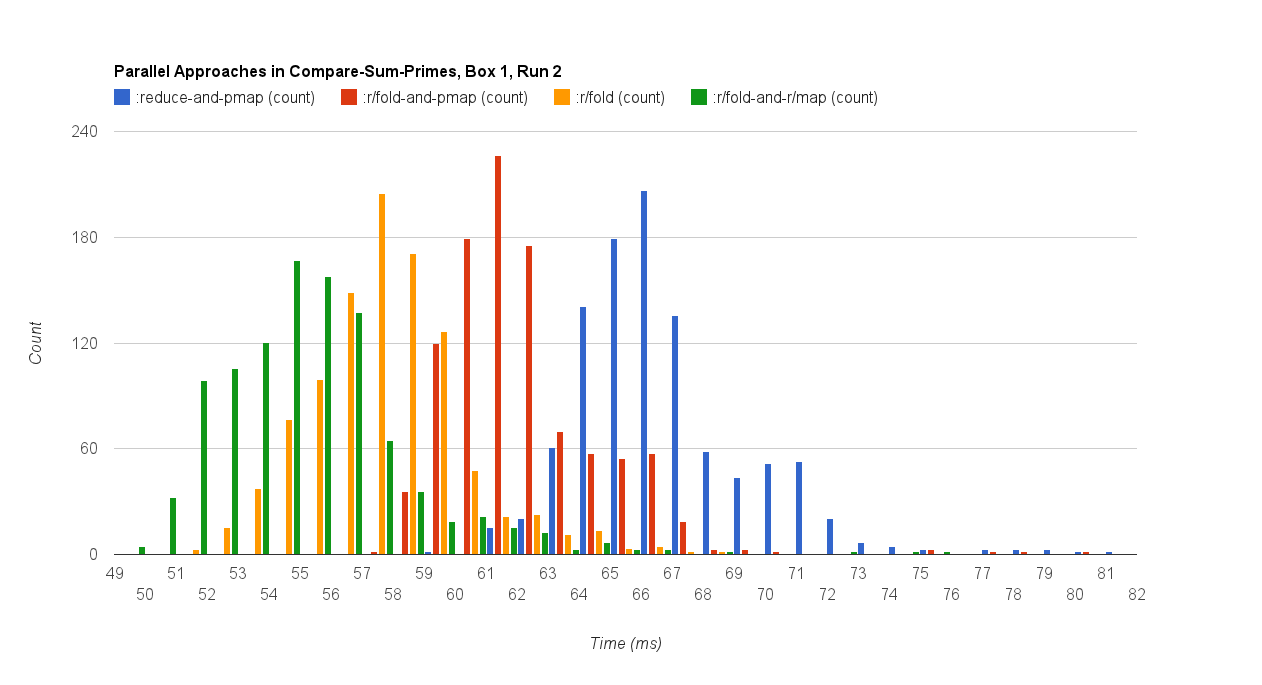
\includegraphics[trim = 10mm 10mm 30mm 30mm, clip, width = 16cm,height = 10cm]{PSP-B1}
\caption{Parallel combinations in Compare-Sum-Primes, Box 1, Run 2 (ms)}\label{figure:parallel}
\end{figure}
 Figure~\ref{figure:parallel} shows the distribution of functions that run faster than serial time; because this is Box 1, \clocode{reduce + pmap} and \clocode{r/fold + pmap} are running properly, in parallel.
\begin{figure}[h!]
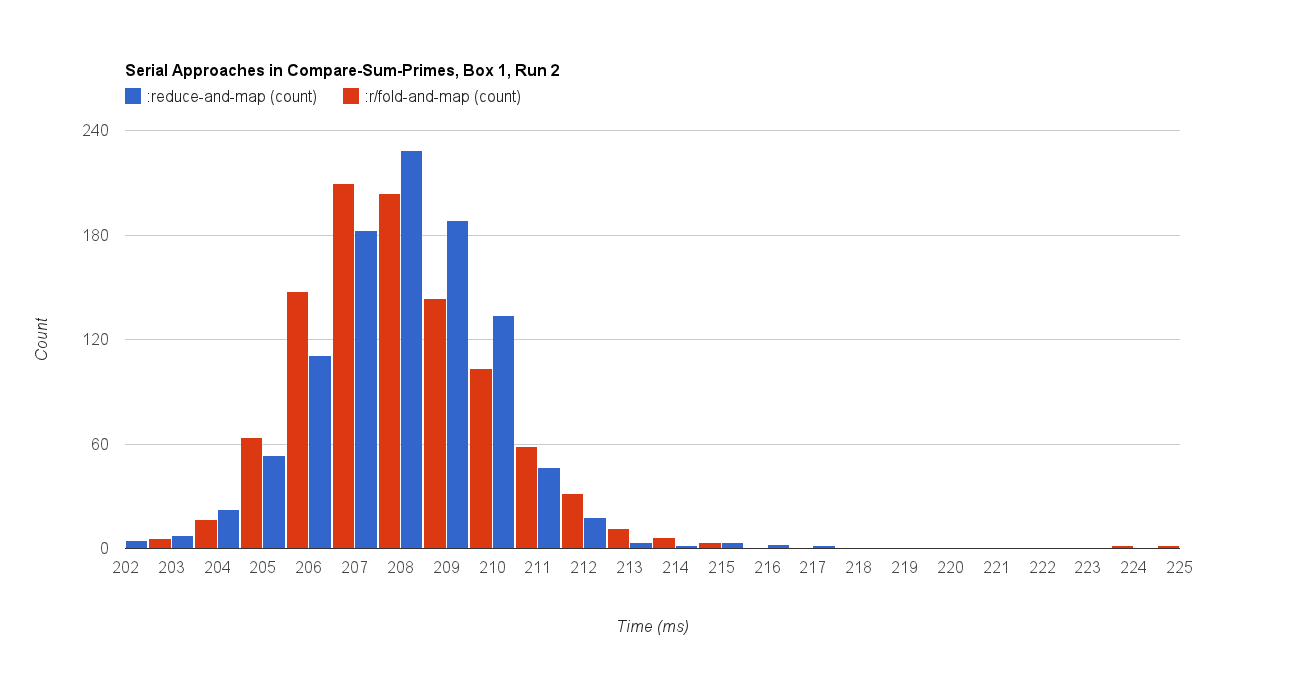
\includegraphics[trim = 10mm 10mm 10mm 30mm, clip, width = 16cm,height = 9.75cm]{SSP-B1}
\caption{Serial combinations in Compare-Sum-Primes, Box 1, Run 2 (ms)}\label{figure:serial}
\end{figure}
Figure~\ref{figure:serial} shows the distribution of functions that run in serial time. Only \clocode{reduce + map} and \clocode{r/fold + map} run in serial time.

A typical mode was to find that the distribution was in two peaks - the serial methods and the parallel methods. Figure~\ref{figure:parallel} is slightly atypical - \clocode{reduce} + \clocode{pmap} was functioning properly, and running in parallel time.

\subsection{Box discussion}\label{sec:boxdiscussion}

\hfcomment{move into discussion?}
\subsubsection{Box 1}

Box 1, with an Intel I7-4700Mq CPU, was the fastest machine tested by a fair margin. It was also the only box where \clocode{pmap} ran faster than \clocode{reduce + map}. We have suspect that \clocode{pmap} is causing thread thrashing, and given that this machine is the only one with hyper-threading, it seems likely that hyperthreading has some effect on the CPU's ability to manage large amounts of threads without thrashing. Reducers ran close to the expected maximum speedup given the number of cores - 300\%.

\subsubsection{Box 2}

Box 2, with an Intel I5-650 CPU, was the slowest machine tested. Notably, \clocode{pmap} ran much slower than serial time on compare-sum-sqrt. This machine does not have hyper threading, and \clocode{pmap}'s performance in that test is what lead us on to thread thrashing in the first place. Reducers ran close to the expected maximum speedup given the number of cores - 300\%.

\subsubsection{Box 3}

Box 3 was our only AMD machine, running a fx-8350 CPU. This machine, while also without hyperthreading, still handled \clocode{pmap} better than Box 2. It did not, however, reach the expected speedup - as an 8 core CPU, using reducers should show a 700\% improvement, but it actually ran near a 300\% improvement. The fx-8350 CPU is technically an 8 core CPU; it's architecture, where each pair of cores is packaged into a module that shares some components between cores~\cite{McIntyre:2012}, may have something to do with this.
\subsection{Discussion}\label{sec:discussion}

We have found that the reducers library, in all tested cases, reduces the execution time significantly. In both Intel machines, the reduction was close to a factor of the number of cores. The AMD fx-8350 machine tested did not show this same pattern. We suspect that the somewhat novel Bulldozer architecture, where each pair of cores is packaged into modules that share components~\cite{McIntyre:2012},  was a factor. 

Combining reducers functions, such as \clocode{r/fold} + \clocode{r/map}, runs within a standard error of the one-step \clocode{r/fold} method. It seems likely that they have the same, or approximately the same runtime. This was expected since, as we discussed in Section~\ref{sec:reducers}, reducers perform all their operations in a single parallel traversal of a collection. 

There are a few interesting observations about \clocode{pmap} based on our results. Firstly, configurations with \clocode{pmap} perform the same, regardless of whether a serial \clocode{reduce} or a parallel \clocode{r/fold} was used. This implies that the collection returned by \clocode{pmap} was not suited for optimizations performed by \clocode{r/fold}. 
There is a variety of collection types, with various degree of laziness, that can be returned from a mapping function. 
Further studies are needed to determine the exact collection type and how it affects the subsequent application of reduction. 
One should note that \clocode{pmap} and reducers were never designed to work together, so it is not surprising that the benefits of  \clocode{pmap} do not prompt benefits of \clocode{r/fold}. 

Another curious observation about  \clocode{pmap} is that it can produce running times ranging from close to the best parallel runs (such as just r/fold configuration) to times worse than serial. In its best results \clocode{reduce} + \clocode{pmap} ran much faster than serial time, and was still slower than reducers only by 15\%. However, in the worst cases  \clocode{pmap} was up to 244\% slower than serial methods. We observed that  \clocode{pmap} generates a large thread poll, so thread thrashing (see Section~\ref{sec;reducers}) is a likely explanation for this slow-down. Unless one has fine-grained control over the number of threads \clocode{pmap} generates, it is difficult to predict whether using  \clocode{pmap} would be beneficial for a given problem on a given machine. 

%We briefly looked into the cause, but were unable to gather a statistically significant amount of data. What data we do have points to a large amount of threads being created, leading to excessive context switching. When \clocode{pmap} was working, \clocode{reduce} + \clocode{pmap} ran faster than serial time, but was still slower than reducers by 15\%. The simplest description of \clocode{pmap} is inconsistency - there is no obvious way to predict whether \clocode{pmap} will run properly on a given machine. Beneficial performance of \clocode{pmap} seem to be correlated with computationally expensive mapping operations (which is not surprising), but more studies would be needed to conclude this with certainty. 

\section{Conclusions and future work}\label{sec:conclusion}




\subsection{Future Work}\label{sec:future}
During our study, we found a number of issues we were unable to address - the most visible of which is the poor performance of \clocode{pmap} - finding that a parallel function is slower than a serial function is unexpected, to say the least. While we do have a hypothesis as to why we see this behavior, we do not have enough information to conclude our hypothesis is correct. Reducers gives us another round of questions; how does reducers decide how many threads it creates? Is there an optimal number of threads? What effect does CPU architecture have on Clojure's concurrency?	
These questions have major implications toward the usage of Clojure reducers and \clocode{pmap} in production environments; \clocode{pmap} has significant qualifiers that need to be addressed in order to produce effective code.

\section{Acknowledgments} 
The authors thank Jon Anthony for helpful discussions and methodology suggestions. 




%
% The following two commands are all you need in the
% initial runs of your .tex file to
% produce the bibliography for the citations in your paper.
%\bibliographystyle{abbrv}
%\end{thebibliography}




%\bibliography{generic_types}  
% You must have a proper ".bib" file
%  and remember to run:
% latex bibtex latex latex
% to resolve all references
%
% ACM needs 'a single self-contained file'!
%
\bibliographystyle{abbrv}
\bibliography{mics2014reducers}








% That's all folks!
\end{document}

%%%%%%%%%%%%%%%%%%%%%%%%%%%%%%%%%%%%%%%%%%%%%%%%%%%%%%%%%%%%%%%%
